% \section{Introduction}

% Distributed training and inference place communication squarely on the critical path alongside computation~\cite{megatron-lm, nanoflow}.
% \saurabh{First bring overlap say to reduce impact of communication on critical path first overlap was built. To further enhance recently new libraries and hardware works}
% The systems community has recognized this and responded with remarkable progress. Device-initiated communication interfaces---NVSHMEM~\cite{nvshmem} and NCCL's device-side APIs~\cite{nccl_deviceapi}---enabled fine-grained overlap between compute and collectives, and expert-crafted libraries such as DeepEP~\cite{deepep2025}, FLUX~\cite{chang2024flux}, and TokenWeave~\cite{gond2025tokenweave} demonstrated the substantial performance gains that become possible when the two are co-designed inside a single kernel.

% The landscape, however, evolves rapidly. New GPU architectures, new communication primitives, new model structures with novel communication patterns (\eg Mixture-of-Experts all-to-all~\cite{deepep2025}), and diverse deployment topologies (NVLink, InfiniBand, RoCE, PCIe) continously alter the co-design trade-offs \saurabh{try to end the sentence with impact, facts and then say something like requiring kernel developers to continously evolve to achive high efficiency}. Today's workloads' expert written kernels are necessarily tuned for specific configurations---and that specificity is precisely what makes them fast \saurabh{move the sentence towards later, first state problem with continous evolution. When you have highlighted all the problems, large space, modern ML compiler, then say something along the lines while bespoke solutions with manual effort maybe possible continously adapting them requires balancing this vast trade-off, making it challenging, time consuming and limited to few experts }. The challenge is that the pace of change means the community continually needs new co-designed solutions, while navigating the complex interplay of tiling, synchronization, chunk sizing, and stream topology~\cite{chang2024flux, zheng2025tilelink} remains an arduous, time-consuming manual task.


% Modern ML compilers offer limited relief: they assume communication lives outside the kernel boundary~\cite{triton, xla, zheng2025tilelink}, and moving it inside violates the assumptions underlying operator scheduling and memory-access planning~\cite{10.1109/SC41406.2024.00094}.

% To address this bottleneck, we bring agentic AI to the co-design process. Given a host-driven baseline \saurabh{again host-driven baseline, what is this, never introduced before } and an LLM API key\saurabh{what is the significan of LLM api key}, \cufuse{} generates co-designed compute--communication kernels that outperform or closely approach hand-tuned quality, discovering configurations empirically per topology.


% \saurabh{What is fused kernel, introduced first time here , average neurips reviewer might not know fused kernels, put something in the first paragraph.}
% Naively prompting an LLM to produce fused kernels fails catastrophically: our ablation shows that skipping a 
% \saurabh{not sure if you should throw a number that early, we haven't introduced evolution, what is evolution budget, what are broken candidates? a reader at this point doesn't have any idea of these terms.}
% correctness-first stage wastes over 25\% of the evolution budget on broken candidates that never compile or deadlock at runtime. The systems community needs a principled recipe. \cufuse{} provides one through three inter-twined components:
% \begin{enumerate}[leftmargin=1.4em,itemsep=1pt,topsep=2pt]
%   \item A \emph{structured design space} that constrains the agent's degrees of freedom to valid communication primitives, synchronization patterns, and tiling strategies---grounding reasoning in collective semantics rather than free-form code generation.
%   \item A \emph{correctness-first fast path} that composes computation and communication into barrier-delimited phases, producing a reliable baseline before any optimization begins.
%   \item A \emph{performance-driven slow path} that uses evolution-style search with empirical hardware feedback (latency etc.) to explore overlap strategies, chunk granularities, and stream topologies, converging on high-performance implementations tailored to each workload and hardware context.
% \end{enumerate}

% A key insight underlying \cufuse{} is that expert communication libraries and co-design frameworks address complementary layers of the problem. Libraries like DeepEP provide highly optimized communication primitives, yet higher-level co-design decisions---overlap strategy, stream topology, chunk granularity---are left to the user. \cufuse{} automates exactly this layer. On intranode MoE dispatch, \cufuse{}'s automatically discovered two-stream overlap pipeline matches DeepEP's end-to-end execution time---not by achieving faster raw communication, but by finding a co-design strategy that hides communication behind compute. An expert could build the same pipeline on top of DeepEP's primitives; \cufuse{} discovers it without manual effort, and adapts it to new topologies automatically.

% Our contributions are as follows:
% \begin{enumerate}[leftmargin=1.4em,itemsep=1pt,topsep=2pt]
%   \item \textbf{Structured design-space formalization.} We define a minimal, declarative set of communication primitive choices that makes compute--communication co-design tractable for LLM agents. Existing expert systems~\cite{deepep2025, chang2024flux, gond2025tokenweave} can be expressed as points in this space.
%   \item \textbf{Two-phase agentic pipeline.} We introduce a fast-path/slow-path recipe---correctness first, then evolution-driven performance search---as a general methodology for agent-driven optimization.
%   \saurabh{strong emperical results are not a contribution, that is basic necessity}
%   \item \textbf{Strong empirical results.} \cufuse{} matches or closely approaches hand-tuned expert libraries on co-designed workloads and delivers up to $1.57\times$ speedup over host-driven baselines, at an LLM cost under \$10 per workload.
% \end{enumerate}

% \cufuse{} is implemented in 18K lines of Python and evaluated on four classes of multi-GPU kernels spanning AllReduce, AllGather, ReduceScatter, and All-to-All collectives. To support the community and accelerate progress on compute--communication co-design, we will fully open-source \cufuse{}.

% \saurabh{Ping me once you have fixed the intro, i think flow is pretty decent most of the place, needs to be careful when writin terms. Good job. }

\vspace{-8pt}
\section{Introduction}
\vspace{-8pt}

In distributed training and inference, communication sits squarely on the critical path alongside computation~\cite{megatron-lm, nanoflow}. To mitigate these communication bottlenecks, researchers have proposed techniques such as compression, overlap, and diverse forms of parallelism. However, recent systems like DeepEP~\cite{deepep2025} and Flux~\cite{chang2024flux} demonstrate that the latency of launching communication kernels has rapidly become a dominant overhead.

% -keeps communication outside the kernel boundary, 
% limiting overlap to coarse-grained pipelining across CUDA streams. 
To overcome this limitation, GPU vendors have upended traditional host-driven communication—where the CPU launches all kernels—by enabling device-initiated execution. Interfaces such as NVSHMEM~\cite{nvshmem} and NCCL's device-side APIs~\cite{nccl_deviceapi} allow GPU threads to issue network requests directly from within a compute kernel, facilitating fine-grained interleaving at the tile or warp level. However, this architectural shift introduces a complex new design space. To effectively overlap computation and communication, developers must now make intricate decisions regarding the underlying communication backend, synchronization primitives, issuer granularity, and transfer placement. While expert-crafted libraries like DeepEP~\cite{deepep2025}, FLUX~\cite{chang2024flux}, and TokenWeave~\cite{gond2025tokenweave} manually navigate this space to achieve substantial speedups, their optimizations remain tightly coupled to specific workloads and network topologies.

\begin{figure*}[t]
\centering
\begin{minipage}[t]{0.48\textwidth}
    \centering
    \setlength{\abovecaptionskip}{2pt}
    \setlength{\belowcaptionskip}{-10pt}
    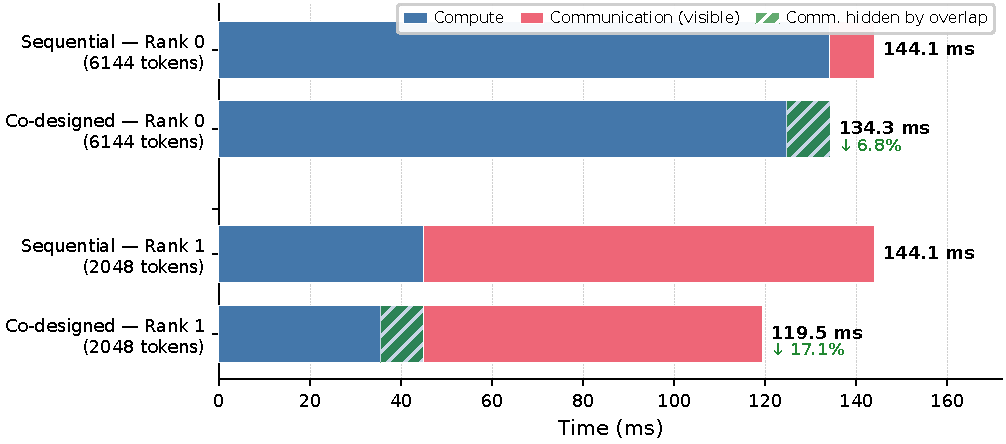
\includegraphics[width=\linewidth]{images/motivation_breakdown.pdf}
    \caption{\small{\textbf{Why co-design matters.} Per-rank latency breakdown of a DeepSeek-V3 MoE layer (2 GPUs, inter-node).}}
    \label{fig:motivation}
\end{minipage}\hfill
\begin{minipage}[t]{0.48\textwidth}
    \centering
    \setlength{\abovecaptionskip}{2pt}
    \setlength{\belowcaptionskip}{-10pt}
    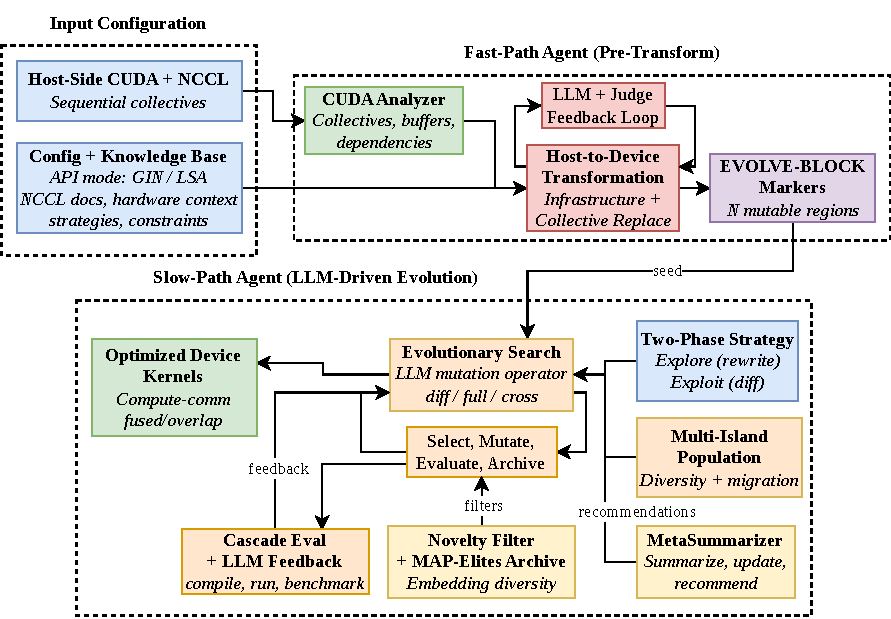
\includegraphics[width=\linewidth]{images/workflow_temp_2.pdf}
    \caption{\small{Overall workflow of \cufuse{}.}}
    \label{fig:workflow}
\end{minipage}
\vspace{-17pt}
\end{figure*}

% The landscape, however, evolves rapidly. New GPU architectures, new communication primitives, new model structures with novel communication patterns (\eg Mixture-of-Experts all-to-all~\cite{deepep2025}), and diverse deployment topologies (NVLink, InfiniBand, RoCE, PCIe) continuously alter the co-design trade-offs, requiring constant rewrites of kernels to maintain high efficiency. Modern ML compilers offer limited relief: they assume communication lives outside the kernel boundary~\cite{triton, xla, zheng2025tilelink}, and moving it inside violates the assumptions underlying operator scheduling and memory-access planning~\cite{10.1109/SC41406.2024.00094}. While bespoke, expert-written kernels are tuned for specific configurations---and that specificity is precisely what makes them fast---adapting them to new workloads and deployments requires balancing a vast design space across tiling, synchronization, chunk sizing etc.~\cite{chang2024flux, zheng2025tilelink}. This makes the continuous development of new co-designed solutions a very arduous and time-consuming manual task.

However, this design space is highly volatile. Evolving hardware generations, diverse interconnect topologies (such as NVLink, InfiniBand, RoCE, and PCIe), and emerging model architectures with novel communication patterns (\eg, Mixture-of-Experts all-to-all~\cite{deepep2025}) constantly shift the optimal design parameters. Consequently, maintaining efficiency across varying deployments requires frequent, manual kernel rewrites. Figure~\ref{fig:motivation} illustrates this concretely: during a DeepSeek-V3 MoE layer, communication consumes up to 69\% of the wall time on lightly-loaded ranks, yet a carefully co-designed strategy—overlapping dispatch with compute using variable-size transfers—can reduce end-to-end latency by 7--17\%. Unfortunately, modern ML compilers offer no relief. They assume communication occurs strictly outside the kernel boundary~\cite{triton, xla, zheng2025tilelink}; migrating it inside violates their foundational assumptions for operator scheduling and memory-access planning~\cite{10.1109/SC41406.2024.00094}. While bespoke, expert-written kernels achieve high performance by rigorously tuning for specific configurations, adapting them to new workloads demands navigating a massive design space of tiling, synchronization, and chunk sizing~\cite{chang2024flux, zheng2025tilelink}. This complexity restricts effective co-design to a small fraction of developers with deep systems expertise. Furthermore, these highly tuned stacks frequently rely on specific assumptions—such as the presence of RDMA or particular NVLink topologies—that are absent in many computing clusters, preventing practitioners from utilizing a single, drop-in library across heterogeneous environments~\cite{deepep2025, licker2025rdmap2p}.


However, new GPU generations and evolving interconnects like NVLink, Infiniband etc  change the choice of design parameters. New model structures introduce novel communication patterns (\eg Mixture-of-Experts all-to-all~\cite{deepep2025}), and deployment topologies vary across NVLink, InfiniBand, RoCE, and PCIe---each altering the co-design trade-offs and requiring kernel rewrites to maintain efficiency. Figure~\ref{fig:motivation} illustrates this concretely: on the DeepSeek-V3 MoE layer, communication consumes up to 69\% of wall time on the lightly-loaded rank, yet carefully co-designed strategies---overlapping dispatch with compute, using variable-size transfers---can reduce end-to-end latency by 7--17\%. Modern ML compilers offer no relief: they assume communication lives outside the kernel boundary~\cite{triton, xla, zheng2025tilelink}, and moving it inside violates the assumptions underlying operator scheduling and memory-access planning~\cite{10.1109/SC41406.2024.00094}. While bespoke, expert-written kernels are tuned for specific configurations---and that specificity is precisely what makes them fast---adapting them to new workloads and deployments requires balancing a large design space across tiling, synchronization, chunk sizing etc.~\cite{chang2024flux, zheng2025tilelink}, limiting co-design to developers with deep systems expertise. Moreover, existing stacks often assume NVLink, RDMA, GPU generations and specific topology configurations that are absent on many computing clusters, so practitioners cannot drop in the same library everywhere~\cite{deepep2025, licker2025rdmap2p}.

To address this bottleneck, we bring agentic AI to the co-design process. Given a host-driven baseline---where the CPU launches communication between compute kernels---our framework, \cufuse{}, automatically transforms it into a device-initiated kernel where GPU threads issue communication from within the compute code. The framework navigates the device-side design space (backend, placement, synchronization, granularity) to automatically discover high-performing configurations for each target topology.

\noindent\textbf{Target regime.} Co-design yields the largest gains when communication is on the critical path, when orchestration overhead is amplified across repeated exchanges (e.g., ring attention with many rounds) etc. Conversely, co-design is less likely to help when compute dominates wall time, when intra-node NVLink bandwidth makes communication negligible, or when an expert library already exposes the right fused schedule for the target workload and topology. \cufuse{} is designed for the former regime.

Naively prompting an LLM to produce co-designed kernels is inefficient, as it often generates candidates that fail to compile or deadlock at runtime. To make agentic co-design practical, the community needs a principled recipe. \cufuse{} provides one through three inter-twined components:
\begin{enumerate}[leftmargin=1.4em,itemsep=1pt,topsep=2pt]
  \item A \emph{structured design space} that constrains the agent's degrees of freedom to valid communication primitives, synchronization patterns, and tiling strategies---grounding reasoning in collective semantics rather than free-form code generation.
  \item A \emph{correctness-first fast path} that composes computation and communication into barrier-delimited phases, producing a reliable baseline before any optimization begins.
  \item A \emph{performance-driven slow path} that uses evolution-style search with empirical hardware feedback (latency etc.) to explore overlap strategies, chunk granularities, and stream topologies, converging on high-performance implementations tailored to each workload and hardware context.
\end{enumerate}

\vspace{-4pt}
A key insight underlying \cufuse{} is that expert communication libraries address a complementary layer of the problem. Libraries like DeepEP provide highly optimized communication primitives and even expose async APIs and multi-stream building blocks, yet the higher-level co-design decisions that determine end-to-end performance (overlap strategy, self/remote compute decomposition, stream topology, backend selection) are left to the user. \cufuse{} automates exactly this layer: for example, on intranode MoE dispatch, it discovers a two-stream overlap pipeline that hides dispatch behind local-chunk compute, a composition an expert could build manually on top of DeepEP's primitives.

Our contributions are as follows:
\vspace{-4pt}

\begin{enumerate}[leftmargin=1.4em,itemsep=1pt,topsep=2pt]
  \item \textbf{LLMs as bounded operators over domain-defined search spaces.} We formalize a structured configuration space for compute-communication co-design that constrains LLM agents to valid primitives, synchronization patterns, and tiling strategies. Existing expert systems~\cite{deepep2025, chang2024flux} can be expressed as points in this space. Without this structure, agents default to unconstrained code generation and repeatedly produce broken or suboptimal kernels.
  \item \textbf{Correctness-first decomposition for agentic optimization.} We introduce a fast-path/slow-path pipeline that separates correctness (constrained transformation to a verified seed) from performance (evolutionary search).
  \item \textbf{Portability through injected context, not retraining.} \cufuse{} adapts across intra-node (NVLink) and inter-node (InfiniBand) deployments by injecting hardware context into the agent prompt rather than baking topology knowledge into the system. This avoids the fine-tuning cost that limits prior agentic kernel generators~\cite{kevin} to fixed hardware targets.
\end{enumerate}

\cufuse{} is implemented in 18K lines of Python and evaluated on four multi-GPU workloads spanning Flash Attention, MoE dispatch/combine, KV-cache transfer, and GEMM+AllGather. Across these workloads, \cufuse{} achieves up to $1.57\times$ speedup over host-driven baselines. On a DeepSeek-V3 MoE layer, \cufuse{}'s discovered two-stream overlap strategy outperforms standard DeepEP usage by 12\%---not through faster primitives, but by hiding dispatch behind self-compute. All results are achieved at an LLM cost under \$10 per workload. To support the community, we release \cufuse{} as open source: \url{\AnonymousCucoMirrorURL}.

